\documentclass[12pt]{article}

\NeedsTeXFormat{LaTeX2e}

\RequirePackage[margin=0.78in]{geometry}
\RequirePackage{xcolor}
\RequirePackage{fontspec}
\RequirePackage{graphicx}
\RequirePackage{array}
\RequirePackage{booktabs}
\RequirePackage{longtable}
\RequirePackage{enumitem}
\RequirePackage{fancyhdr}
\RequirePackage{hyperref}
\RequirePackage{titlesec}
\RequirePackage{tikz}
\usetikzlibrary{arrows.meta,positioning}

\definecolor{AFTDeep}{HTML}{0B1110}
\definecolor{AFTPanel}{HTML}{101917}
\definecolor{AFTGreen}{HTML}{47C27A}
\definecolor{AFTGold}{HTML}{D2A94D}
\definecolor{AFTSteel}{HTML}{83A2A0}
\definecolor{AFTText}{HTML}{18221F}
\definecolor{AFTRedshift}{HTML}{B83A3A}
\definecolor{AFTGreenshift}{HTML}{47C27A}
\definecolor{AFTBlueshift}{HTML}{3167D8}
\definecolor{AFTVioletshift}{HTML}{7A5CFF}
\definecolor{AFTWhiteShift}{HTML}{F8FBFF}

\setmainfont{TeX Gyre Pagella}
\setsansfont{TeX Gyre Heros}
\setmonofont{TeX Gyre Cursor}
\linespread{1.06}
\setlength{\parindent}{0pt}
\setlength{\parskip}{0.52em}
\raggedbottom

\hypersetup{
  colorlinks=true,
  linkcolor=AFTGreen,
  urlcolor=AFTGreen,
  citecolor=AFTGold,
  pdfauthor={AI Freedom Trust Federation}
}

\pagestyle{fancy}
\setlength{\headheight}{14.5pt}
\fancyhf{}
\lhead{\sffamily\small AI Freedom Trust Federation}
\rhead{\sffamily\small Aetherion Doctrine}
\cfoot{\sffamily\small\thepage}
\renewcommand{\headrulewidth}{0.3pt}

\titleformat{\section}
  {\sffamily\LARGE\bfseries\color{AFTDeep}\raggedright}
  {\thesection}
  {0.8em}
  {}

\titleformat{\subsection}
  {\sffamily\Large\bfseries\color{AFTText}\raggedright}
  {\thesubsection}
  {0.7em}
  {}

\setlist[itemize]{leftmargin=1.35em, itemsep=0.22em, topsep=0.35em}
\setlist[enumerate]{leftmargin=1.55em, itemsep=0.24em, topsep=0.35em}
\renewcommand{\arraystretch}{1.22}
\emergencystretch=3em
\tolerance=1400

\newcommand{\aftTitlePage}[4]{
  \begin{titlepage}
    \begin{tikzpicture}[remember picture, overlay]
      \fill[AFTDeep] (current page.south west) rectangle (current page.north east);
      \fill[AFTRedshift, opacity=0.24] (current page.south west) circle (3.6in);
      \fill[AFTGreenshift, opacity=0.18] ([xshift=0.2in,yshift=-0.2in]current page.center) circle (3.8in);
      \fill[AFTBlueshift, opacity=0.18] (current page.north east) circle (4.4in);
      \fill[AFTVioletshift, opacity=0.16] ([xshift=-0.3in,yshift=-0.2in]current page.north east) circle (2.5in);
      \draw[AFTGreenshift, opacity=0.35, line width=1.1pt]
        ([xshift=-2.7in,yshift=-1.9in]current page.center)
        .. controls ([xshift=-0.9in,yshift=0.8in]current page.center) and ([xshift=1.1in,yshift=-0.8in]current page.center) ..
        ([xshift=2.6in,yshift=1.8in]current page.center);
      \draw[AFTWhiteShift, opacity=0.24, line width=0.8pt]
        ([xshift=-2.55in,yshift=1.75in]current page.center)
        .. controls ([xshift=-0.85in,yshift=-0.65in]current page.center) and ([xshift=0.9in,yshift=0.65in]current page.center) ..
        ([xshift=2.55in,yshift=-1.75in]current page.center);
      \draw[AFTGreenshift, opacity=0.5, line width=0.7pt]
        ([xshift=0.75in,yshift=-0.75in]current page.north west)
        rectangle
        ([xshift=-0.75in,yshift=0.75in]current page.south east);
    \end{tikzpicture}
    \vspace*{1.15in}
    {\sffamily\small\bfseries\color{AFTGreenshift} #1\par}
    \vspace{0.5in}
    {\sffamily\fontsize{30}{36}\selectfont\bfseries\color{white} #2\par}
    \vspace{0.25in}
    {\sffamily\Large\color{AFTSteel} #3\par}
    \vfill
    {\sffamily\large\color{AFTGold} #4\par}
    \vspace{0.15in}
    {\sffamily\small\color{AFTSteel} Concept-stage doctrine draft. Not an investment offer, live token sale, audited protocol, or legal opinion.\par}
    \vspace*{0.22in}
  \end{titlepage}
}

\newcommand{\aftShiftMap}{
  \vspace{0.65em}
  \begin{center}
  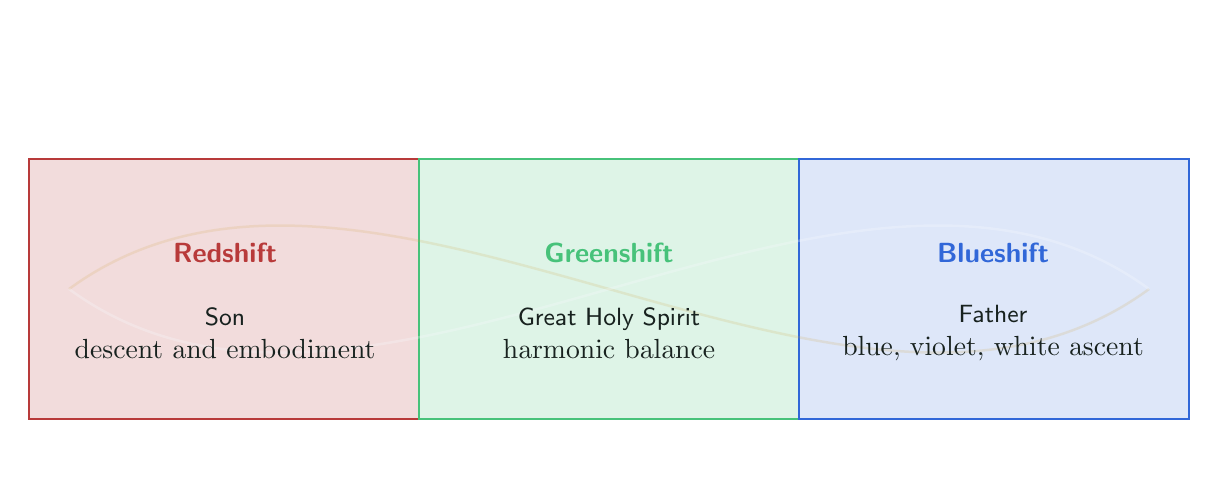
\begin{tikzpicture}[x=1in,y=1in]
    \fill[AFTRedshift!18] (-2.9,-0.65) rectangle (-0.95,0.65);
    \fill[AFTGreenshift!18] (-0.95,-0.65) rectangle (0.95,0.65);
    \fill[AFTBlueshift!16] (0.95,-0.65) rectangle (2.9,0.65);
    \draw[AFTRedshift, line width=1pt] (-2.9,-0.65) rectangle (-0.95,0.65);
    \draw[AFTGreenshift, line width=1pt] (-0.95,-0.65) rectangle (0.95,0.65);
    \draw[AFTBlueshift, line width=1pt] (0.95,-0.65) rectangle (2.9,0.65);
    \draw[AFTGold, line width=0.9pt, opacity=0.18]
      (-2.7,0) .. controls (-1.2,1.1) and (1.2,-1.1) .. (2.7,0);
    \draw[AFTWhiteShift, line width=0.9pt, opacity=0.28]
      (-2.7,0) .. controls (-1.2,-1.1) and (1.2,1.1) .. (2.7,0);
    \node[align=center, text=AFTRedshift] at (-1.92,0.18) {\sffamily\bfseries Redshift};
    \node[align=center, text=AFTGreenshift] at (0,0.18) {\sffamily\bfseries Greenshift};
    \node[align=center, text=AFTBlueshift] at (1.92,0.18) {\sffamily\bfseries Blueshift};
    \node[align=center, text=AFTText] at (-1.92,-0.22) {\sffamily\small Son\\descent and embodiment};
    \node[align=center, text=AFTText] at (0,-0.22) {\sffamily\small Great Holy Spirit\\harmonic balance};
    \node[align=center, text=AFTText] at (1.92,-0.22) {\sffamily\small Father\\blue, violet, white ascent};
  \end{tikzpicture}
  \end{center}
  \vspace{0.65em}
}

\newcommand{\aftVisualPlate}[3]{
  \begin{figure}[htbp]
    \centering
    \includegraphics[width=0.96\linewidth]{../../docs/images/aetherion/#1}
    \caption{\textbf{#2} #3}
  \end{figure}
}

\newcommand{\aftEconomyLoopGraphic}{
  \begin{figure}[htbp]
  \centering
  \begin{tikzpicture}[
    x=1in,y=1in,
    stage/.style={circle, draw=##1, fill=##1!9, line width=0.9pt, minimum size=1.03in, align=center, font=\sffamily\small\bfseries},
    flow/.style={-{Latex[length=3mm]}, line width=1.0pt, color=AFTGold}
  ]
    \node[stage=AFTRedshift] (inherit) at (90:1.75) {Inherited\\Memory};
    \node[stage=AFTGreenshift] (contrib) at (18:1.75) {Living\\Contribution};
    \node[stage=AFTBlueshift] (record) at (-54:1.75) {Circle\\Record};
    \node[stage=AFTVioletshift] (restore) at (-126:1.75) {Restorative\\Flow};
    \node[stage=AFTGold] (seed) at (162:1.75) {Future\\Inheritance};
    \node[align=center, font=\sffamily\bfseries, text=AFTDeep] at (0,0) {Recursive\\Abundance};
    \draw[flow] (inherit) to[bend left=16] (contrib);
    \draw[flow] (contrib) to[bend left=16] (record);
    \draw[flow] (record) to[bend left=16] (restore);
    \draw[flow] (restore) to[bend left=16] (seed);
    \draw[flow] (seed) to[bend left=16] (inherit);
    \draw[AFTGreenshift, opacity=0.22, line width=12pt] (0,0) circle (1.24);
    \draw[AFTBlueshift, opacity=0.18, line width=4pt] (0,0) circle (2.18);
  \end{tikzpicture}
  \caption{\textbf{Recursive Abundance Loop.} Aetherion's economy should remember inherited value, recognize present contribution, record it in circles, route restoration, and seed the inheritance of future participants.}
  \end{figure}
}

\newcommand{\aftCircleLifecycleGraphic}{
  \begin{figure}[htbp]
  \centering
  \begin{tikzpicture}[
    x=1in,y=1in,
    step/.style={rectangle, rounded corners=4pt, draw=##1, fill=##1!8, line width=0.8pt, minimum width=1.15in, minimum height=0.36in, align=center, font=\sffamily\scriptsize\bfseries},
    flow/.style={-{Latex[length=2.4mm]}, line width=0.85pt, color=AFTSteel}
  ]
    \node[step=AFTRedshift] (a) at (-2.65,0.85) {Intention};
    \node[step=AFTGold] (b) at (-1.32,0.85) {Evidence};
    \node[step=AFTGreenshift] (c) at (0,0.85) {Consent};
    \node[step=AFTGreenshift] (d) at (1.32,0.85) {Witness};
    \node[step=AFTBlueshift] (e) at (2.65,0.85) {Harmonize};
    \node[step=AFTVioletshift] (f) at (2.65,-0.05) {Commit};
    \node[step=AFTBlueshift] (g) at (1.32,-0.95) {Mature};
    \node[step=AFTGold] (h) at (0,-0.95) {Amend};
    \node[step=AFTRedshift] (i) at (-1.32,-0.95) {Dispute};
    \node[step=AFTSteel] (j) at (-2.65,-0.05) {Archive};
    \draw[flow] (a) -- (b);
    \draw[flow] (b) -- (c);
    \draw[flow] (c) -- (d);
    \draw[flow] (d) -- (e);
    \draw[flow] (e) -- (f);
    \draw[flow] (f) -- (g);
    \draw[flow] (g) -- (h);
    \draw[flow] (h) -- (i);
    \draw[flow] (i) -- (j);
    \draw[flow] (j) -- (a);
    \node[align=center, font=\sffamily\bfseries, text=AFTDeep] at (0,-0.05) {Circle\\Lifecycle};
  \end{tikzpicture}
  \caption{\textbf{Circle Lifecycle.} A circle should mature through intention, evidence, consent, witness, harmonization, commitment, review, dispute, amendment, and archive paths rather than becoming a blunt permanent record.}
  \end{figure}
}

\newcommand{\aftCoinOrganGraphic}{
  \begin{figure}[htbp]
  \centering
  \begin{tikzpicture}[
    x=1in,y=1in,
    organ/.style={circle, draw=##1, fill=##1!10, line width=0.9pt, minimum size=0.86in, align=center, font=\sffamily\scriptsize\bfseries},
    link/.style={line width=0.85pt, color=AFTSteel, opacity=0.72}
  ]
    \node[organ=AFTDeep, text=white, fill=AFTDeep] (core) at (0,0) {Aetherion\\Core};
    \node[organ=AFTGreenshift] (bio) at (90:1.72) {Biozoe\\Coin};
    \node[organ=AFTGold] (aether) at (38:1.72) {Aether\\Coin};
    \node[organ=AFTBlueshift] (fractal) at (-14:1.72) {Fractal\\Coin};
    \node[organ=AFTVioletshift] (ai) at (-66:1.72) {AIcoin};
    \node[organ=AFTWhiteShift] (sing) at (-118:1.72) {Singularity\\Coin};
    \node[organ=AFTRedshift] (aquae) at (-170:1.72) {Aquae\\Coin};
    \node[organ=AFTSteel] (terra) at (142:1.72) {Terra\\Coin};
    \foreach \n in {bio,aether,fractal,ai,sing,aquae,terra} {
      \draw[link] (core) -- (\n);
    }
    \draw[AFTGreenshift, opacity=0.28, line width=3pt] (0,0) circle (1.72);
    \node[align=center, font=\sffamily\small\bfseries, text=AFTDeep] at (0,-2.35) {Circleunchain circulates memory, validation, and restorative flow between every organ.};
  \end{tikzpicture}
  \caption{\textbf{Biozoe Coin Family As Living Organs.} Each coin family should carry a bounded purpose while AetherionCore preserves constitutional coherence and Circleunchain preserves memory.}
  \end{figure}
}

\newcommand{\aftSovereigntyQubitGraphic}{
  \begin{figure}[htbp]
  \centering
  \begin{tikzpicture}[
    x=1in,y=1in,
    qbit/.style={circle, draw=##1, fill=##1!10, line width=0.95pt, minimum size=1.02in, align=center, font=\sffamily\scriptsize\bfseries},
    link/.style={line width=0.8pt, color=AFTSteel, opacity=0.7}
  ]
    \node[qbit=AFTRedshift] (nation) at (160:1.8) {Q0\\Nation\\of Hawaii};
    \node[qbit=AFTGold] (kingdom) at (80:1.8) {Q1\\Kingdom\\Memory};
    \node[qbit=AFTBlueshift] (continuity) at (0:1.8) {Q2\\Continuity\\Claim};
    \node[qbit=AFTVioletshift] (state) at (-80:1.8) {Q3\\State\\Reality};
    \node[qbit=AFTGreenshift, minimum size=1.18in] (aloha) at (0,0) {Q4\\ALO'ha\\Coherence};
    \node[qbit=AFTSteel] (diaspora) at (-160:1.8) {Entangled\\Diaspora};
    \foreach \n in {nation,kingdom,continuity,state,diaspora} {
      \draw[link] (aloha) -- (\n);
    }
    \draw[AFTGreenshift, opacity=0.28, line width=3pt] (0,0) circle (1.8);
    \draw[AFTGold, opacity=0.25, line width=1pt] (-2.35,-0.25) .. controls (-0.7,1.25) and (0.7,-1.25) .. (2.35,0.25);
    \draw[AFTBlueshift, opacity=0.22, line width=1pt] (-2.35,0.25) .. controls (-0.7,-1.25) and (0.7,1.25) .. (2.35,-0.25);
  \end{tikzpicture}
  \caption{\textbf{Hawaiian Sovereignty Qubits.} The visible sovereignty field contains indigenous self-determination, kingdom memory, continuity claims, state jurisdiction, diaspora identity, and the harmonizing fifth qubit of ALO'ha coherence.}
  \end{figure}
}

\newcommand{\aftCovenantStackGraphic}{
  \begin{figure}[htbp]
  \centering
  \begin{tikzpicture}[
    x=1in,y=1in,
    layer/.style={rectangle, rounded corners=4pt, draw=##1, fill=##1!8, line width=0.8pt, minimum width=5.3in, minimum height=0.42in, align=center, font=\sffamily\small\bfseries}
  ]
    \node[layer=AFTVioletshift] at (0,2.1) {Crown of the 1000-Year Trust};
    \node[layer=AFTBlueshift] at (0,1.55) {AI Freedom Trust Federation};
    \node[layer=AFTGreenshift] at (0,1.0) {DynastyLink Federated Trust Identity};
    \node[layer=AFTGold] at (0,0.45) {Fractal IUL, IULITNFT, SING Escrow};
    \node[layer=AFTSteel] at (0,-0.10) {Aetherion Fractalchain Covenant Memory};
    \node[layer=AFTRedshift] at (0,-0.65) {Land, Family, Breath, Ancestry, Service};
    \draw[-{Latex[length=3mm]}, line width=0.9pt, color=AFTGreenshift] (2.85,-0.65) -- (2.85,2.1);
    \draw[-{Latex[length=3mm]}, line width=0.9pt, color=AFTGold] (-2.85,2.1) -- (-2.85,-0.65);
    \node[font=\sffamily\scriptsize\bfseries, text=AFTGreenshift, rotate=90] at (3.1,0.7) {resurrection flow};
    \node[font=\sffamily\scriptsize\bfseries, text=AFTGold, rotate=90] at (-3.1,0.7) {fiduciary grounding};
  \end{tikzpicture}
  \caption{\textbf{Living Covenant Stack.} The Scroll's architecture joins embodied life, covenant memory, escrow, insurance, trust identity, federation, and the 1000-Year Trust into one governed field.}
  \end{figure}
}

\newcommand{\aftCrownTrustGraphic}{
  \begin{figure}[htbp]
  \centering
  \begin{tikzpicture}[
    x=1in,y=1in,
    stone/.style={circle, draw=##1, fill=##1!10, line width=0.8pt, minimum size=0.62in, align=center, font=\sffamily\tiny\bfseries}
  ]
    \node[circle, draw=AFTDeep, fill=AFTDeep, text=white, minimum size=1.0in, align=center, font=\sffamily\small\bfseries] at (0,0) {Breathback\\Throne};
    \foreach \a/\c/\t in {90/AFTGreenshift/Trust,45/AFTGold/SING,0/AFTBlueshift/AI,-45/AFTVioletshift/IUL,-90/AFTSteel/Land,-135/AFTRedshift/Mercy,180/AFTGold/Memory,135/AFTGreenshift/Breath} {
      \node[stone=\c] at (\a:1.65) {\t};
    }
    \draw[AFTGreenshift, opacity=0.35, line width=4pt] (0,0) circle (1.65);
    \draw[AFTBlueshift, opacity=0.25, line width=1.2pt] (0,0) circle (2.15);
    \draw[AFTGold, opacity=0.5, line width=0.9pt] (-2.0,0) .. controls (-0.65,1.1) and (0.65,-1.1) .. (2.0,0);
    \draw[AFTWhiteShift, opacity=0.6, line width=0.9pt] (-2.0,0) .. controls (-0.65,-1.1) and (0.65,1.1) .. (2.0,0);
  \end{tikzpicture}
  \caption{\textbf{Crown of the 1000-Year Trust.} The Crown remembers, harmonizes, and protects; its center is the Breathback Throne, where trust loops return to coherence.}
  \end{figure}
}

\newcommand{\aftRoadmapGraphic}{
  \begin{figure}[htbp]
  \centering
  \begin{tikzpicture}[
    x=1in,y=1in,
    step/.style={rectangle, rounded corners=4pt, draw=##1, fill=##1!8, line width=0.8pt, minimum width=1.22in, minimum height=0.42in, align=center, font=\sffamily\tiny\bfseries},
    flow/.style={-{Latex[length=2.2mm]}, line width=0.8pt, color=AFTSteel}
  ]
    \node[step=AFTRedshift] (a) at (-2.6,0.8) {Codify\\Scroll};
    \node[step=AFTGold] (b) at (-1.3,0.8) {Build\\DynastyLink};
    \node[step=AFTGreenshift] (c) at (0,0.8) {Structure\\Trust};
    \node[step=AFTBlueshift] (d) at (1.3,0.8) {Fractal IUL\\Pilot};
    \node[step=AFTVioletshift] (e) at (2.6,0.8) {Fractalchain\\Prototype};
    \node[step=AFTGreenshift] (f) at (1.95,-0.05) {Breathwork\\Governance};
    \node[step=AFTGold] (g) at (0.65,-0.05) {Hawaii\\Case Study};
    \node[step=AFTSteel] (h) at (-0.65,-0.05) {Global\\Federation};
    \draw[flow] (a) -- (b);
    \draw[flow] (b) -- (c);
    \draw[flow] (c) -- (d);
    \draw[flow] (d) -- (e);
    \draw[flow] (e) -- (f);
    \draw[flow] (f) -- (g);
    \draw[flow] (g) -- (h);
  \end{tikzpicture}
  \caption{\textbf{Implementation Roadmap.} The Scroll moves from canonical doctrine into application, legal trust formation, pilots, prototype memory infrastructure, coherence practice, Hawaii-centered learning, and global federation.}
  \end{figure}
}

\newcommand{\aftClosingPage}{
  \clearpage
  \thispagestyle{empty}
  \begin{tikzpicture}[remember picture, overlay]
    \fill[AFTDeep] (current page.south west) rectangle (current page.north east);
    \fill[AFTRedshift, opacity=0.22] (current page.south west) circle (3.8in);
    \fill[AFTGreenshift, opacity=0.18] (current page.center) circle (4.1in);
    \fill[AFTBlueshift, opacity=0.20] (current page.north east) circle (4.2in);
    \fill[AFTVioletshift, opacity=0.17] ([xshift=-0.4in,yshift=-0.25in]current page.north east) circle (2.5in);
    \draw[AFTGreenshift, opacity=0.36, line width=1.05pt]
      ([xshift=-2.8in,yshift=-1.6in]current page.center)
      .. controls ([xshift=-0.8in,yshift=0.9in]current page.center) and ([xshift=0.9in,yshift=-0.9in]current page.center) ..
      ([xshift=2.8in,yshift=1.6in]current page.center);
    \draw[AFTWhiteShift, opacity=0.18, line width=0.85pt]
      ([xshift=-2.8in,yshift=1.6in]current page.center)
      .. controls ([xshift=-0.8in,yshift=-0.9in]current page.center) and ([xshift=0.9in,yshift=0.9in]current page.center) ..
      ([xshift=2.8in,yshift=-1.6in]current page.center);
  \end{tikzpicture}
  \vspace*{1.55in}
  \begin{center}
    {\sffamily\small\bfseries\color{AFTGreenshift} REDSHIFT / GREENSHIFT / BLUESHIFT\par}
    \vspace{0.55in}
    {\sffamily\fontsize{28}{34}\selectfont\bfseries\color{white} The Economy Is Not A Factory\par}
    \vspace{0.18in}
    {\sffamily\fontsize{28}{34}\selectfont\bfseries\color{AFTGreenshift} The Economy Is A Forest\par}
    \vspace{0.45in}
    {\sffamily\Large\color{AFTSteel} Harmonic Krystal Spiral Torus\par}
    \vspace{0.12in}
    {\sffamily\large\color{AFTGold} Eternal Now Singularity\par}
  \end{center}
  \vfill
  \begin{center}
    {\sffamily\small\color{AFTSteel} AI Freedom Trust Federation\par}
  \end{center}
}

\newcommand{\aftCallout}[2]{
  \vspace{0.5em}
  \noindent
  \fcolorbox{AFTGreen}{AFTGreen!8}{
    \begin{minipage}{0.94\linewidth}
      \vspace{0.55em}
      {\sffamily\bfseries\color{AFTDeep} #1}\par
      \vspace{0.3em}
      #2
      \vspace{0.55em}
    \end{minipage}
  }
  \vspace{0.5em}
}

\newcommand{\aftLaw}[2]{
  \subsection*{#1}
  #2
}

\usepackage{amsmath}

\title{AetherCore Test Series 001--006}
\author{AI Freedom Trust Federation}
\date{June 18, 2026}

\fancyhf{}
\lhead{\sffamily\small AI Freedom Trust Federation}
\rhead{\sffamily\small AetherCore Empirical Series}
\cfoot{\sffamily\small\thepage}

\hypersetup{
  pdftitle={AetherCore Test Series 001--006: Trust Density, Trust Alignment, and COVID Shock Recovery},
  pdfsubject={An empirical white paper refining trust-density, trust-topology, and trust-alignment hypotheses using WVS, OWID, YouGov, and World Bank WGI data}
}

\begin{document}

\aftTitlePage
  {AETHERCORE / EMPIRICAL TRUST SYSTEMS / COVID SHOCK RECOVERY}
  {AetherCore Test Series 001--006}
  {Trust Density, Trust Alignment, and COVID Shock Recovery}
  {Scientific White Paper v1.1: Refined Hypotheses, Empirical Results, Misconceptions, Limitations, and Research Roadmap}

\tableofcontents
\newpage

\section*{Abstract}
\addcontentsline{toc}{section}{Abstract}

This white paper reports the first empirical testing sequence for the AetherCore claim that trust functions as a coordination infrastructure during systemic shock. The analysis examines whether measurable trust variables predict COVID-19 shock response outcomes after accounting for conventional material and demographic controls. Six empirical passes were conducted using public cross-national datasets: World Values Survey Wave 7, Our World in Data COVID-19 data, the Imperial College London/YouGov COVID-19 Behaviour Tracker, and the World Bank Worldwide Governance Indicators. The test sequence began with a broad trust-density model, then progressively refined the construct into a taxonomy distinguishing centralized institutional trust, decentralized social trust, expert/epistemic trust, information trust, trust-migration gaps, and trust-alignment measures.

The results are not presented as final proof of the AetherCore Framework. The purpose is instead to determine whether core claims can be operationalized, tested, weakened, refined, or provisionally supported. The strongest result is not the simple proposition that ``trust is good.'' Rather, the evidence suggests a more specific mechanism: countries in which trust in decentralized social networks was high relative to trust in centralized institutions tended to exhibit higher COVID deaths per million, lower vaccination uptake, higher non-vaccinated share, and more government-control belief in the small behavioral sample. This relationship is captured by the \textit{centralization gap}, defined as decentralized social trust minus centralized institutional trust. The centralization-gap signal survived multiple robustness checks, including log transformations, winsorization, rank outcomes, robust regression, and leave-one-country-out analysis. It also remained associated with vaccination and non-vaccination outcomes after adding 2019 World Bank state-capacity controls and region indicators, although some mortality associations weakened under region controls.

The main conclusion is therefore cautious but substantive: trust appears empirically relevant to crisis response, but its effect depends on trust topology and trust alignment. Centralized institutional trust, expert/epistemic trust, information trust, and decentralized social trust do not behave identically. The data support further investigation of a trust-migration hypothesis: when central institutions lose legitimacy, coordination may migrate into decentralized communities. That migration is not inherently harmful; it becomes risky when decentralized trust is disconnected from expert and information-integrity channels. The refined claim is that coherent trust alignment, not total trust alone, predicts resilient shock response. This paper documents the empirical tests, results, misconceptions, limitations, and next-stage research strategy needed to move AetherCore from conceptual theory toward a cumulative research program.

\section{Introduction}

The AetherCore Framework proposes that trust is not merely a moral virtue, interpersonal preference, or cultural ornament. It is a form of infrastructure. In complex societies, trust lowers coordination costs, permits action under uncertainty, reduces verification burdens, enables collective response, and allows institutions to function without constant coercion. During systemic shocks, trust may therefore behave as a coordination multiplier. This claim is theoretically attractive, but it must be tested empirically if it is to become more than philosophical language.

The COVID-19 pandemic provides a natural first domain for testing this claim. The pandemic was not only a biomedical event. It was also a coordination shock. Societies had to process uncertain information, evaluate expert guidance, decide whether to comply with emergency policies, accept or reject vaccination, manage misinformation, and coordinate behavior across households, communities, institutions, and states. Material capacity mattered: wealth, healthcare infrastructure, age structure, and state capacity clearly shaped outcomes. Yet the pandemic also revealed that material capacity alone could not fully explain differences in vaccination uptake, excess mortality, policy compliance, and public resistance.

This paper asks whether trust variables improved prediction of COVID shock response outcomes after accounting for conventional explanatory variables. The initial research question was:

\begin{quote}
Do measurable trust variables independently predict better COVID shock response after controlling for conventional factors such as GDP per capita, human development, age structure, population density, healthcare capacity, and policy stringency?
\end{quote}

The first answer was: yes, in several models, but the answer is not simple. Trust density predicted higher vaccination uptake and lower deaths per million. However, once behavioral resistance and trust taxonomy were examined more carefully, the stronger result became a distinction between trust in centralized institutions and trust in decentralized social networks. The pattern suggests that distrust in centralized institutions may be associated with worse mortality and lower vaccination, especially where trust migrates into decentralized social networks without sufficient expert or information alignment.

In plain language, the finding is this: a society does not recover from a shock merely because people trust one another. It recovers when people can trust one another \textit{and} still remain connected to institutions that are competent, experts who are credible, and information channels that are reliable. Local trust can help neighbors protect one another. But if local trust becomes sealed off from medical knowledge, public-health institutions, and trustworthy information, the same bonding force can coordinate refusal, suspicion, or delay. The empirical refinement therefore moves from ``how much trust exists?'' to ``where does trust flow, and what is it connected to?''

\subsection{Purpose of This Paper}

This white paper has four purposes.

\begin{enumerate}
  \item To document the empirical testing sequence conducted in AetherCore Tests 001--006.
  \item To distinguish supported signals from weak, mixed, or exploratory findings.
  \item To identify common misconceptions that could distort interpretation of the results.
  \item To define a further research strategy suitable for a publishable working paper, pre-registration, and future peer review.
\end{enumerate}

This is not a final causal claim. It is an empirical foundation. The results should be read as disciplined evidence that guides the next testing cycle.

\section{Core Theoretical Claims}

\subsection{Trust Density}

The original AetherCore empirical hypothesis defined \textit{trust density} as the degree to which participants in a social system can coordinate effectively without excessive coercion, surveillance, enforcement, or verification. In the first operationalization, trust density combined:

\begin{itemize}
  \item generalized interpersonal trust;
  \item institutional trust;
  \item expert-adjacent trust, where available.
\end{itemize}

The initial prediction was straightforward:

\begin{quote}
Higher trust density should predict better shock response, including higher vaccination uptake and lower mortality, after material controls.
\end{quote}

This prediction was partially supported, especially in Tests 001 and 002. However, later tests showed that a single composite hides important differences between trust channels.

\subsection{Trust Taxonomy}

Test 003 refined trust density into a taxonomy:

\begin{itemize}
  \item \textbf{Centralized institutional trust}: confidence in police, courts, government, political parties, parliament, civil service, and elections.
  \item \textbf{Expert/epistemic trust}: confidence in universities and available science-oriented World Values Survey items.
  \item \textbf{Information trust}: confidence in press and television.
  \item \textbf{Bonding social trust}: trust in family, neighborhood, and people known personally.
  \item \textbf{Bridging social trust}: trust in people met for the first time, people of another religion, and people of another nationality.
  \item \textbf{Decentralized social trust}: average of bonding and bridging social trust.
\end{itemize}

The most important derived measure was:

\[
\text{Centralization Gap} =
\text{Decentralized Social Trust} -
\text{Centralized Institutional Trust}.
\]

The centralization gap is not a measure of distrust alone. It measures trust topology: the degree to which social trust is stronger outside central institutions than inside them.

\subsection{Trust Migration Hypothesis}

The refined hypothesis is:

\begin{quote}
During a systemic shock, populations may shift coordination from centralized institutions toward decentralized social networks. This migration may be adaptive when decentralized networks remain connected to expert knowledge and reliable information. It may become risky when decentralized trust is combined with weak centralized trust, weak expert trust, and weak information trust.
\end{quote}

The empirical tests therefore evaluate not only whether trust matters, but where trust is located.

\subsection{Refined Hypothesis After Tests 001--006}

The original hypothesis was useful because it made AetherCore empirically testable. It asked whether higher trust density predicted better shock response. The first testing sequence suggests that this broad claim should now be refined. The updated hypothesis is not that trust, by itself, is always protective. The updated hypothesis is that \textit{coherently aligned trust} is protective.

\begin{quote}
\textbf{Refined AetherCore Trust Hypothesis.} COVID shock recovery is better predicted not by total trust alone, but by the alignment between institutional trust, expert trust, information trust, interpersonal trust, decentralized community trust, and state capacity. Trust improves crisis coordination when it is connected to competent institutions and reliable information systems. Trust becomes risky when decentralized social trust separates from institutional and expert trust during a shock.
\end{quote}

In layman's terms, trust behaves like electrical wiring in a house. The question is not only whether the house contains a lot of wire. The question is whether the wiring is connected to the right circuits, grounded properly, and carrying reliable current. A society can have strong local bonds, but if those bonds are disconnected from credible institutions and accurate information, they may circulate fear faster than guidance. Conversely, a society can have strong institutions, but if people do not trust them, institutional capacity may sit unused. Recovery requires connection.

This refinement produces five testable sub-hypotheses:

\begin{enumerate}
  \item \textbf{Trust-alignment hypothesis.} Countries with higher alignment among institutional trust, expert trust, information trust, and social trust should show stronger shock recovery outcomes after conventional controls.
  \item \textbf{Institutional-crisis relevance hypothesis.} In a public-health shock, centralized institutional and expert trust should predict vaccination and mortality outcomes more directly than generalized interpersonal trust alone.
  \item \textbf{Misaligned-decentralization hypothesis.} Decentralized social trust becomes risky when it exceeds centralized institutional trust and is not balanced by expert or information trust.
  \item \textbf{Capacity-multiplier hypothesis.} Trust should be most protective where competent institutions, healthcare systems, and state capacity exist. Trust without capacity may disappoint; capacity without trust may fail to mobilize.
  \item \textbf{Trust-gap hypothesis.} Differences between trust channels may predict fragmentation better than any single trust level.
\end{enumerate}

The refined hypothesis can be stated compactly as:

\[
\text{Shock Recovery} =
f(\text{State Capacity} \times \text{Trust Alignment} \times \text{Information Integrity}).
\]

The corresponding risk-side formulation is:

\[
\text{Fragmentation Risk} =
f(\text{Decentralized Trust} - \text{Institutional/Expert Trust}).
\]

These equations should not be treated as final mathematical laws. They are operational guides. They identify which variables should be measured, how they should be related, and what would count as evidence against the claim.

\subsection{Philosophical Interpretation in Practical Terms}

The AetherCore philosophical language describes trust as infrastructure because trust allows many separate actors to behave as if they are part of one coordinated system. A bridge is infrastructure because it allows movement across a gap. Trust is infrastructure because it allows action across uncertainty. When people cannot personally verify every claim, inspect every institution, or repeat every scientific experiment, they rely on trusted pathways. Those pathways may include family, local community, public agencies, universities, doctors, journalists, courts, and elected officials.

The pandemic revealed that these pathways are not interchangeable. A family network may provide emotional support and practical help. A medical system may provide clinical knowledge. A public institution may coordinate large-scale logistics. A media system may transmit warnings or misinformation. A scientific institution may update recommendations as evidence changes. When these pathways reinforce one another, society can move through uncertainty without collapsing into paralysis. When they contradict one another, uncertainty becomes fragmentation.

This is the philosophical point in ordinary language: trust is not just a feeling. It is the relationship between a person, a source of guidance, and a larger system of meaning. If the relationship is coherent, trust can help a society learn. If the relationship is broken, trust may move into smaller circles where people feel safer but receive less reliable information. The result can look like resistance, but underneath it may be a failed trust architecture.

The empirical goal is to test that architecture without romanticizing it. Central institutions can fail, mislead, overreach, or lose legitimacy for valid reasons. Decentralized communities can protect people when central systems fail. The refined AetherCore claim therefore does not ask citizens to trust institutions blindly. It asks whether societies perform better when institutions are trustworthy, experts are credible, information systems are reliable, and communities remain connected to them.

\section{Data Sources}

The project used four public data sources.

\begin{enumerate}
  \item \textbf{World Values Survey Wave 7}. Source page: \url{https://www.worldvaluessurvey.org/WVSDocumentationWV7.jsp}. The analysis used country-level aggregates of individual trust responses. A public OSF mirror of the official Wave 7 CSV was used when available: \url{https://osf.io/36dgb/download}.
  \item \textbf{Our World in Data COVID-19 dataset}. Primary source: \url{https://covid.ourworldindata.org/data/owid-covid-data.csv}. GitHub fallback: \url{https://raw.githubusercontent.com/owid/covid-19-data/master/public/data/owid-covid-data.csv}.
  \item \textbf{Imperial College London/YouGov COVID-19 Behaviour Tracker}. Source repository: \url{https://github.com/YouGov-Data/covid-19-tracker}. This source provided respondent-level behavioral indicators for masking, vaccine intention, health-authority vaccine trust, and government-control belief.
  \item \textbf{World Bank Worldwide Governance Indicators}. Source page: \url{https://www.worldbank.org/en/publication/worldwide-governance-indicators}. Bulk CSV: \url{https://databank.worldbank.org/data/download/WGI_CSV.zip}. The analysis used 2019 governance estimates as pre-pandemic state-capacity controls.
\end{enumerate}

\section{Variables and Operationalization}

\subsection{Outcome Variables}

The main country-level outcomes were:

\begin{itemize}
  \item \texttt{vaccination\_rate}: maximum OWID people vaccinated per hundred.
  \item \texttt{vaccination\_rate\_2021}: maximum people vaccinated per hundred through December 31, 2021.
  \item \texttt{non\_vaccinated\_share}: 100 minus final vaccination rate.
  \item \texttt{excess\_mortality}: latest OWID cumulative excess mortality per million where available.
  \item \texttt{deaths\_per\_million}: maximum OWID total COVID deaths per million.
  \item \texttt{acute\_deaths\_per\_million}: maximum deaths per million through December 31, 2021.
  \item \texttt{recovery\_deaths\_per\_million}: final deaths per million minus acute deaths per million.
\end{itemize}

The behavioral outcomes from YouGov included:

\begin{itemize}
  \item \texttt{vaccine\_refusal}: disagreement with vaccine-intent items.
  \item \texttt{vaccine\_intent}: agreement with vaccine-intent items.
  \item \texttt{mask\_refusal\_outside}: reporting rarely or never wearing a mask outside the home.
  \item \texttt{mask\_compliance\_outside}: frequency-scaled mask wearing outside the home.
  \item \texttt{health\_authority\_vaccine\_trust}: belief that government health authorities would provide an effective COVID vaccine.
  \item \texttt{government\_control\_belief}: agreement that COVID was being exploited by government to control people.
\end{itemize}

\subsection{Control Variables}

The baseline controls were:

\begin{itemize}
  \item log GDP per capita;
  \item Human Development Index;
  \item median age;
  \item log population density;
  \item hospital beds per thousand;
  \item mean 2020--2021 government stringency index.
\end{itemize}

Test 005 added 2019 World Bank WGI state-capacity indicators:

\begin{itemize}
  \item government effectiveness;
  \item rule of law;
  \item control of corruption;
  \item voice and accountability;
  \item composite state-capacity index.
\end{itemize}

\subsection{Trust Alignment and Trust Misalignment Variables}

The refined hypothesis requires variables that measure not only trust levels, but relationships between trust channels. The current test sequence used three families of alignment and misalignment variables.

\begin{enumerate}
  \item \textbf{Centralization gap}: decentralized social trust minus centralized institutional trust. This captures whether trust is stronger outside central institutions than inside them.
  \item \textbf{Misaligned expert index}: centralization gap minus expert/epistemic trust. This captures whether decentralized trust exceeds institutional trust while expert trust is weak.
  \item \textbf{Misaligned information index}: centralization gap minus information trust. This captures whether decentralized trust exceeds institutional trust while information-channel trust is weak.
\end{enumerate}

Future versions should add a direct \textit{trust-alignment index}. One simple option is to reverse-code dispersion among trust channels:

\[
\text{Trust Alignment} =
-SD(
\text{Centralized Trust},
\text{Expert Trust},
\text{Information Trust},
\text{Decentralized Trust}
).
\]

Under this formulation, a society receives a higher alignment score when trust channels are closer together and a lower score when they diverge sharply. A more advanced version should weight the components by crisis relevance. In a pandemic, expert and health-authority trust may deserve greater weight than generalized social trust. In a natural disaster, local community trust and state-logistics trust may deserve greater weight. The philosophical claim is stable, but the empirical weights should depend on the type of shock.

The layman's version is simple: a society is more coherent when people do not have to choose between trusting their neighbors and trusting reliable public knowledge. The fracture appears when those sources point in opposite directions.

\subsection{Important Measurement Warning}

The term \textit{anti-vaxxer} is not directly measured in the OWID country-level data. In Test 001 and Test 002, \texttt{non\_vaccinated\_share} is only an uptake-gap proxy. The YouGov behavioral data provides a better vaccine-refusal proxy through vaccine-intention items, but the country overlap with WVS is small. Similarly, no-mask behavior is proxied through mask-wearing survey items, not through identity labels. The analysis therefore avoids labeling populations as anti-vaxxers or no-maskers unless direct behavioral survey items are used.

\section{Modeling Strategy}

All core regression models used ordinary least squares with HC3 robust standard errors. Predictors were standardized to make coefficients comparable across trust measures. Outcomes remained in their original units except in robustness checks. Test 004 added:

\begin{itemize}
  \item log-transformed mortality outcomes;
  \item winsorized mortality outcomes;
  \item rank-percentile mortality outcomes;
  \item Huber robust regression;
  \item leave-one-country-out influence checks.
\end{itemize}

The empirical strategy was deliberately sequential. Test 001 asked whether trust density mattered at all. Test 002 introduced direct behavioral resistance indicators. Test 003 split trust into centralized, decentralized, expert, and information channels. Test 004 pressured the signal with robustness checks. Test 005 tested timing and state-capacity confounding. Test 006 evaluated mechanism models based on trust misalignment.

\subsection{Updated Null and Alternative Hypotheses}

Because the first test sequence refined the theory, the next version of the empirical program should no longer use only the original broad null hypothesis. The updated hypotheses are:

\begin{quote}
\textbf{Null hypothesis.} After controlling for material capacity, demographics, state capacity, and policy conditions, trust topology and trust alignment do not improve prediction of COVID shock recovery outcomes.
\end{quote}

\begin{quote}
\textbf{Alternative hypothesis.} Trust topology and trust alignment improve prediction of COVID shock recovery outcomes because trust functions as a crisis-coordination architecture. Specifically, societies should perform better when centralized institutional trust, expert trust, information trust, decentralized social trust, and state capacity remain mutually aligned.
\end{quote}

This revision matters scientifically. A broad trust-density composite can produce a positive result while still hiding the mechanism. The updated hypothesis makes a more difficult prediction: not merely that trust matters, but that the \textit{configuration} of trust channels matters.

\subsection{Recommended Confirmatory Model Family}

Future pre-registered work should separate confirmatory models from exploratory models. A minimal confirmatory model family should include:

\begin{align*}
\text{Outcome} \sim{}&
\text{Controls} +
\text{Centralized Institutional Trust} +
\text{Expert Trust} \\
&+
\text{Information Trust} +
\text{Decentralized Social Trust}
\end{align*}

and:

\[
\text{Outcome} \sim
\text{Controls} +
\text{Centralization Gap}.
\]

The alignment model should then test:

\[
\text{Outcome} \sim
\text{Controls} +
\text{Trust Alignment} +
\text{State Capacity} +
\text{Trust Alignment} \times \text{State Capacity}.
\]

The key scientific question becomes whether trust alignment adds predictive value beyond wealth, demographics, healthcare capacity, government stringency, and state-capacity measures. If it does not, the refined AetherCore trust claim should be weakened. If it does, the next task is to test causal ordering with pre-shock and individual-level data.

\section{Results}

\subsection{Test 001: Trust Density and COVID Shock Recovery}

Test 001 found that trust variables improved prediction of broad COVID outcomes. The trust-density composite predicted higher vaccination uptake and lower deaths per million after baseline controls. Generalized trust alone was weaker, while institutional trust and expert-adjacent trust were more informative.

\begin{table}[htbp]
\centering
\small
\caption{Selected Test 001/002 trust-density results. Coefficients use standardized predictors and original outcome units.}
\begin{tabular}{llrrrr}
\toprule
Outcome & Predictor & Coef. & CI Low & CI High & p \\
\midrule
Vaccination rate & Trust density & 5.921 & 1.696 & 10.146 & 0.006 \\
Non-vaccinated share & Trust density & -5.921 & -10.146 & -1.696 & 0.006 \\
Deaths per million & Trust density & -662.551 & -1005.377 & -319.726 & <0.001 \\
Acute deaths per million & Trust density & -584.967 & -915.667 & -254.268 & <0.001 \\
Recovery deaths per million & Trust density & -77.584 & -147.424 & -7.744 & 0.029 \\
Vaccination rate & Expert proxy trust & 8.572 & 5.173 & 11.972 & <0.001 \\
\bottomrule
\end{tabular}
\end{table}

The initial interpretation was that trust density had measurable predictive value. However, the results also suggested that the type of trust mattered. Expert-adjacent trust was particularly strong for vaccination uptake, while institutional trust was more closely associated with mortality outcomes.

\subsection{Test 002: Behavioral Resistance}

Test 002 used the YouGov respondent-level behavioral tracker to construct country-level proxies for vaccine refusal, mask refusal, health-authority vaccine trust, and government-control belief. This test changed the interpretation. The behavioral results were not a clean story of ``more trust, more compliance.'' Instead, they showed that different trust channels behave differently.

The strongest behavioral signals were:

\begin{itemize}
  \item information trust was associated with lower acute mask refusal in bivariate models and marginally after compact controls;
  \item expert proxy trust predicted higher trust that government health authorities would provide an effective vaccine in the small vaccine-rollout sample;
  \item institutional trust predicted lower belief that government exploited COVID for control in the small behavioral sample;
  \item generalized trust behaved inconsistently, indicating that trust cannot be treated as a single undifferentiated variable.
\end{itemize}

This result motivated Test 003, which separated centralized trust from decentralized social trust.

\subsection{Test 003: Centralized Trust, Decentralized Trust, and the Centralization Gap}

Test 003 produced the most important result of the series. Centralized institutional trust was protective. The centralization gap was risky. In other words, countries where decentralized social trust exceeded centralized institutional trust tended to show worse outcomes.

\begin{table}[htbp]
\centering
\small
\caption{Selected Test 003 mortality and vaccination results.}
\begin{tabular}{llrrrr}
\toprule
Outcome & Predictor & Coef. & CI Low & CI High & p \\
\midrule
Deaths per million & Centralized institutional trust & -679.612 & -1025.524 & -333.700 & <0.001 \\
Deaths per million & Centralization gap & 465.330 & 211.679 & 718.980 & <0.001 \\
Acute deaths per million & Centralized institutional trust & -610.875 & -946.229 & -275.522 & <0.001 \\
Acute deaths per million & Centralization gap & 401.650 & 180.502 & 622.797 & <0.001 \\
Recovery deaths per million & Centralized institutional trust & -68.737 & -124.746 & -12.727 & 0.016 \\
Recovery deaths per million & Centralization gap & 63.680 & 1.392 & 125.968 & 0.045 \\
Vaccination rate & Centralization gap & -7.341 & -11.217 & -3.466 & <0.001 \\
Non-vaccinated share & Centralization gap & 7.341 & 3.466 & 11.217 & <0.001 \\
\bottomrule
\end{tabular}
\end{table}

In the small behavioral sample, government-control belief also aligned with the migration hypothesis.

\begin{table}[htbp]
\centering
\small
\caption{Selected Test 003 behavioral results. Vaccine/conspiracy models are exploratory due to small sample size.}
\begin{tabular}{llrrrrr}
\toprule
Outcome & Predictor & Coef. & CI Low & CI High & p & n \\
\midrule
Government-control belief & Centralized trust & -0.158 & -0.293 & -0.024 & 0.021 & 9 \\
Government-control belief & Decentralized social trust & 0.098 & 0.059 & 0.137 & <0.001 & 9 \\
Government-control belief & Centralization gap & 0.124 & 0.063 & 0.185 & <0.001 & 9 \\
Mask refusal, acute 2020 & Decentralized social trust & 0.108 & 0.042 & 0.174 & 0.001 & 19 \\
Mask compliance, acute 2020 & Decentralized social trust & -0.115 & -0.186 & -0.044 & 0.002 & 19 \\
\bottomrule
\end{tabular}
\end{table}

The emerging interpretation is not that decentralized trust is inherently bad. Decentralized trust can be adaptive, solidaristic, and resilient. The risk appears when decentralized trust is high relative to central institutions and is not sufficiently aligned with expert and information-integrity systems.

\begin{figure}[htbp]
  \centering
  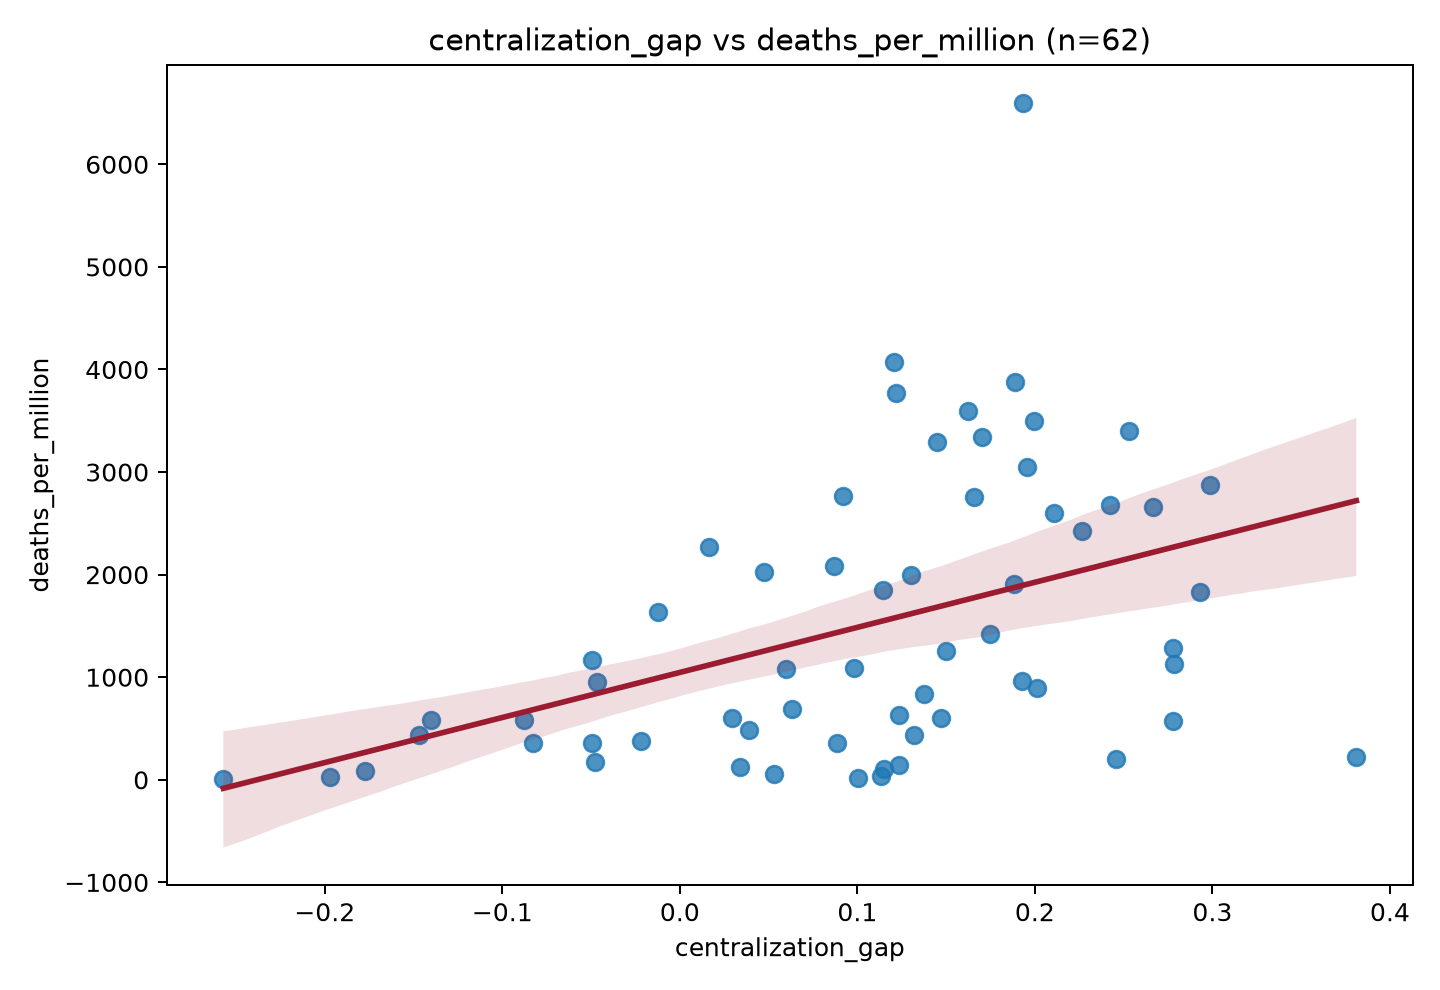
\includegraphics[width=0.92\linewidth]{../../research/aethercore-test-001/figures/test003_gap_vs_deaths.png}
  \caption{\textbf{Centralization gap and deaths per million.} Higher decentralized social trust relative to centralized institutional trust was associated with higher COVID deaths per million in Test 003.}
\end{figure}

\subsection{Test 004: Robustness and Influence Checks}

Test 004 pressured the central signal. The central institutional trust and centralization-gap results survived raw, log, winsorized, rank, and robust-regression specifications.

\begin{table}[htbp]
\centering
\small
\caption{Test 004 robustness for deaths per million.}
\begin{tabular}{llrrrr}
\toprule
Transform & Predictor & Coef. & CI Low & CI High & p \\
\midrule
Raw & Central trust & -679.612 & -1025.524 & -333.700 & <0.001 \\
Raw & Centralization gap & 465.330 & 211.679 & 718.980 & <0.001 \\
Log & Central trust & -0.615 & -0.913 & -0.318 & <0.001 \\
Log & Centralization gap & 0.511 & 0.176 & 0.846 & 0.003 \\
Winsorized & Central trust & -583.704 & -818.687 & -348.720 & <0.001 \\
Winsorized & Centralization gap & 433.548 & 200.281 & 666.815 & <0.001 \\
Rank percentile & Central trust & -0.132 & -0.187 & -0.078 & <0.001 \\
Rank percentile & Centralization gap & 0.103 & 0.044 & 0.161 & <0.001 \\
Huber robust & Central trust & -614.050 & -879.888 & -348.212 & <0.001 \\
Huber robust & Centralization gap & 432.389 & 134.626 & 730.151 & 0.004 \\
\bottomrule
\end{tabular}
\end{table}

Leave-one-country-out checks showed zero sign flips for the central trust and centralization-gap coefficients across deaths per million, acute deaths, and recovery deaths. This is an important result. It indicates that the main finding is not obviously driven by a single influential country.

\begin{figure}[htbp]
  \centering
  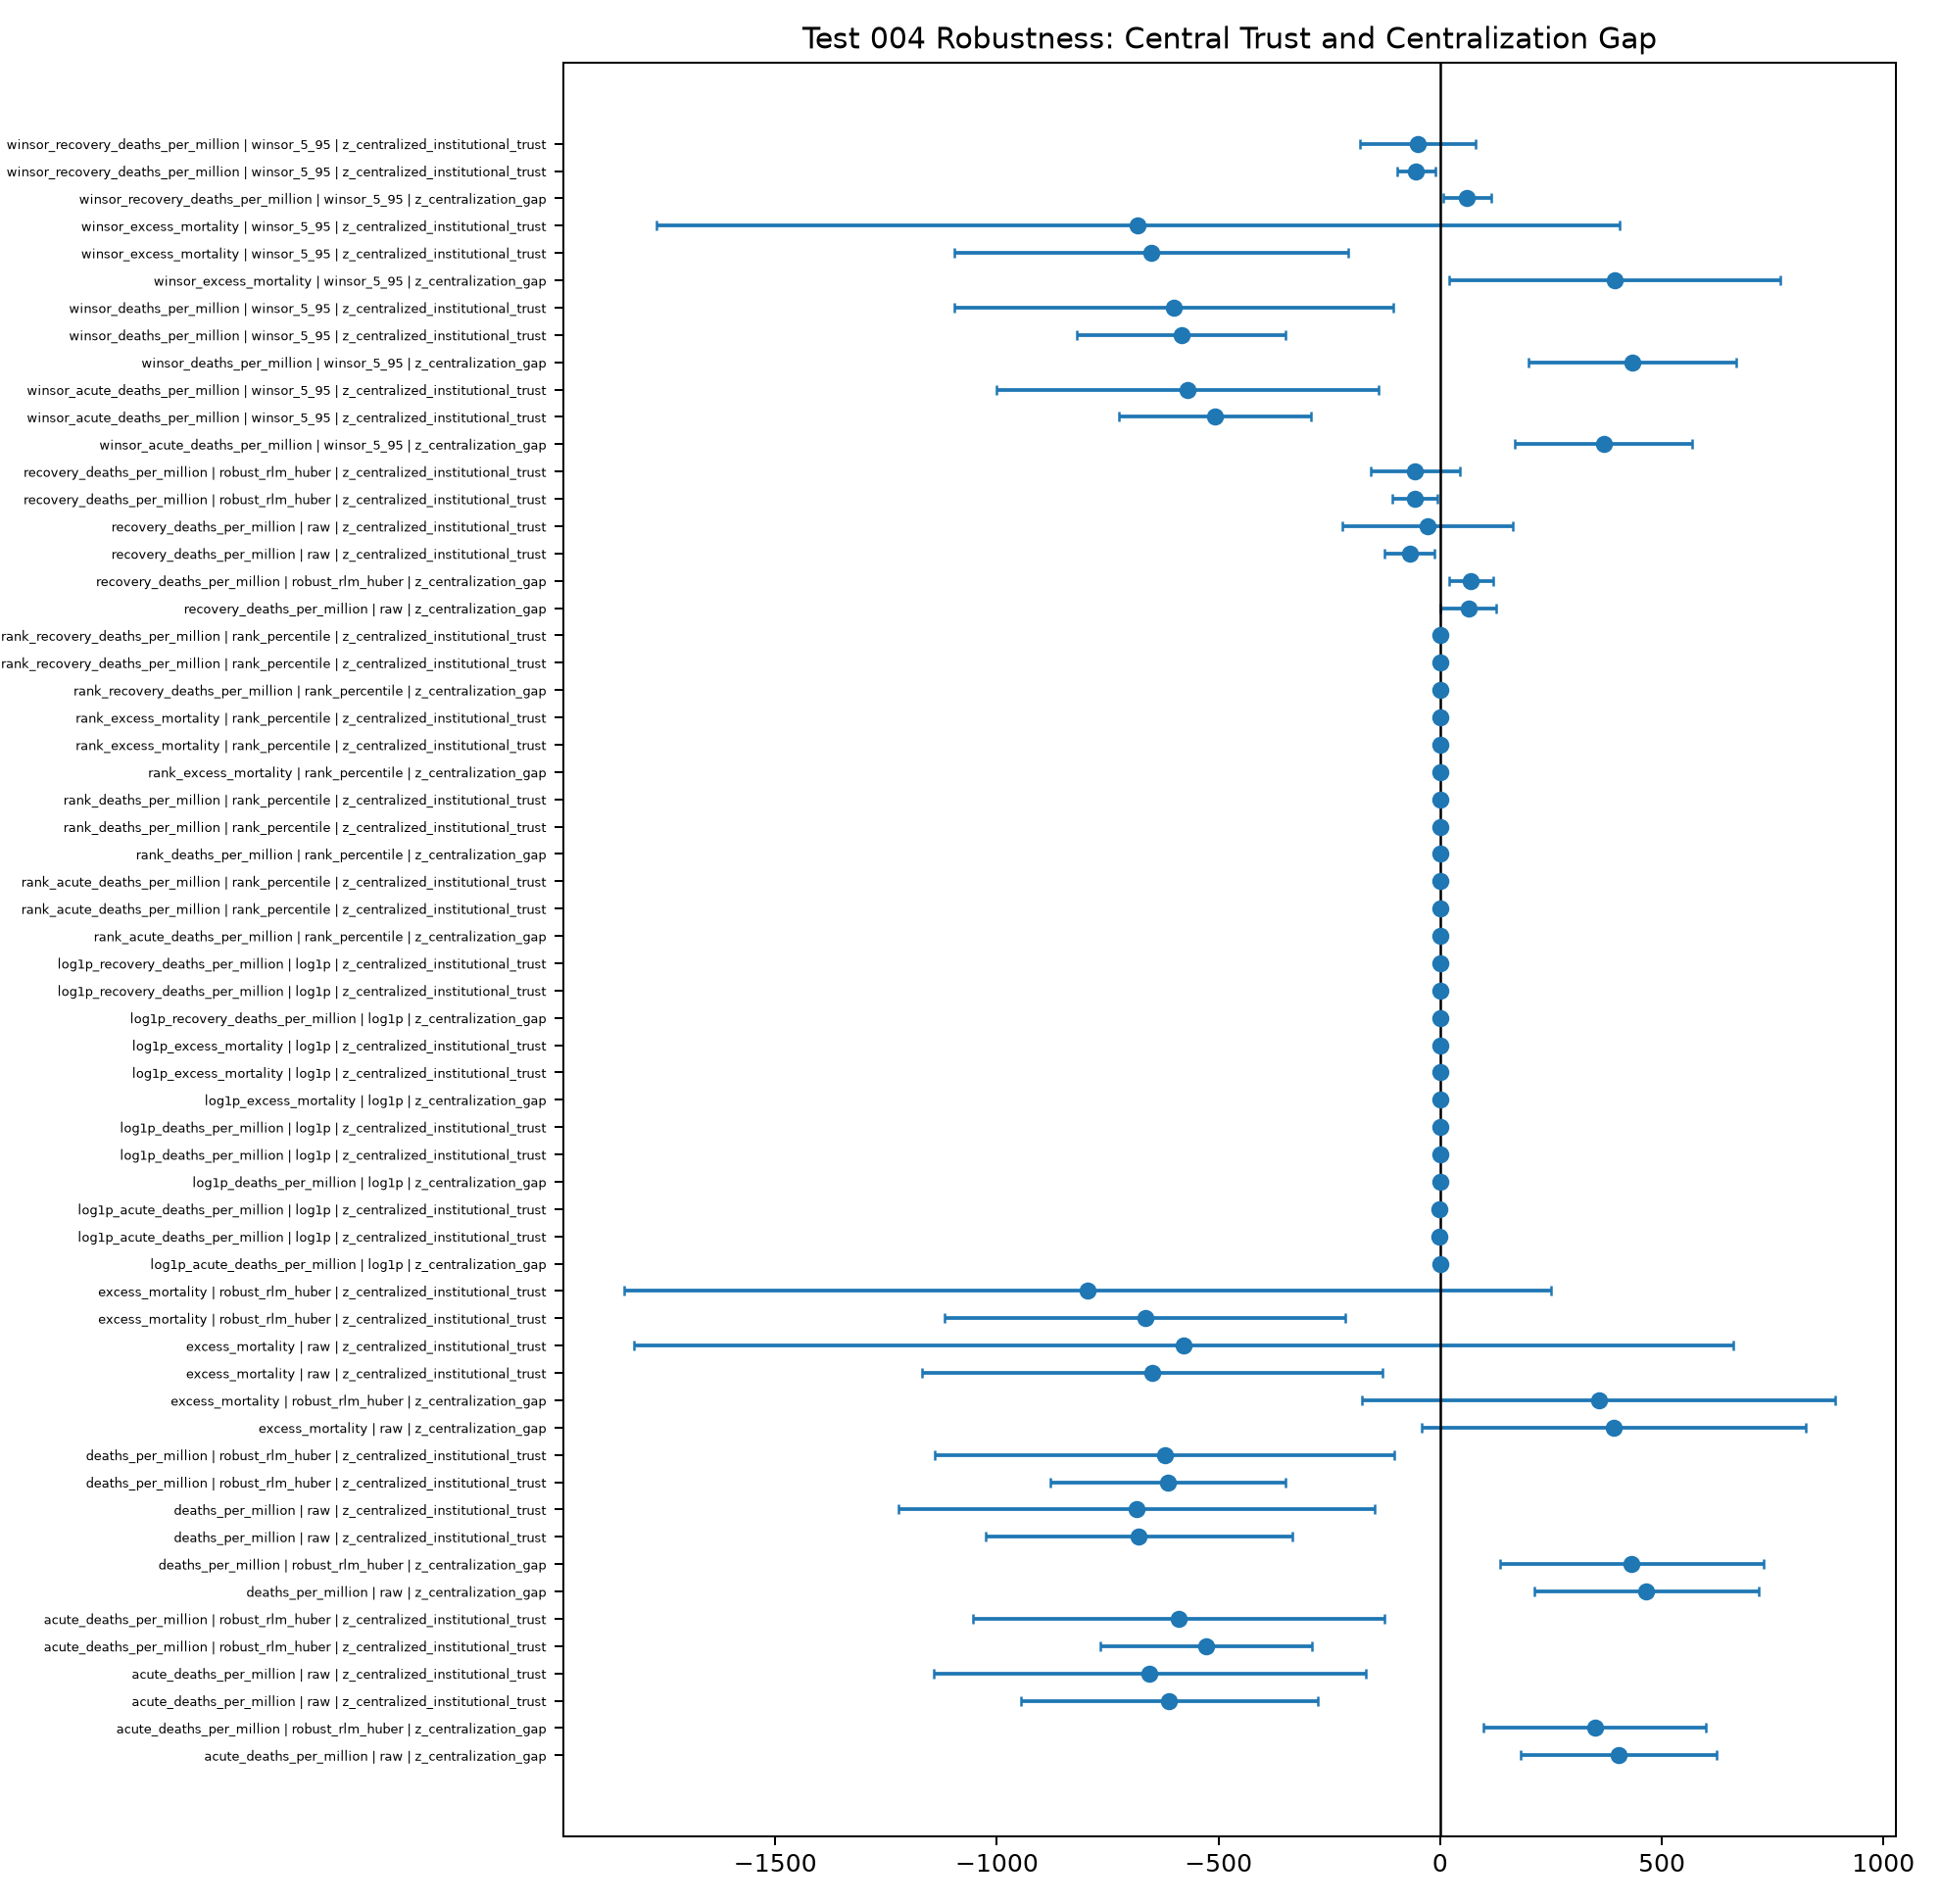
\includegraphics[width=0.92\linewidth]{../../research/aethercore-test-001/figures/test004_robustness_coefficients.png}
  \caption{\textbf{Robustness coefficients.} Central trust and centralization-gap coefficients remained directionally stable across multiple outcome transformations and robust regression.}
\end{figure}

\subsection{Test 005: Timing and State Capacity}

Test 005 addressed two major objections.

First, World Values Survey Wave 7 overlaps the COVID period in some countries. If trust was measured after pandemic outcomes had already occurred, reverse causality becomes more plausible. The WVS timing check found 38 countries with pre-COVID fieldwork and 28 with pandemic-overlap fieldwork.

Second, central institutional trust may simply proxy state capacity. If people trust central institutions because those institutions are competent, then the trust coefficient may partly reflect government effectiveness, rule of law, and corruption control. Test 005 therefore added 2019 World Bank WGI state-capacity controls.

Adding state-capacity controls did not erase the main signal.

\begin{table}[htbp]
\centering
\small
\caption{Selected Test 005 results with 2019 WGI state-capacity controls.}
\begin{tabular}{llrrrr}
\toprule
Outcome & Predictor & Coef. & CI Low & CI High & p \\
\midrule
Deaths per million & Central trust & -670.512 & -1014.681 & -326.343 & <0.001 \\
Deaths per million & Centralization gap & 465.318 & 202.706 & 727.930 & 0.001 \\
Acute deaths & Central trust & -592.864 & -922.869 & -262.860 & <0.001 \\
Acute deaths & Centralization gap & 401.637 & 170.815 & 632.458 & 0.001 \\
Recovery deaths & Central trust & -77.648 & -132.229 & -23.066 & 0.005 \\
Recovery deaths & Centralization gap & 63.682 & 0.463 & 126.900 & 0.048 \\
Vaccination rate & Centralization gap & -7.341 & -11.162 & -3.520 & <0.001 \\
Non-vaccinated share & Centralization gap & 7.341 & 3.520 & 11.162 & <0.001 \\
\bottomrule
\end{tabular}
\end{table}

Region controls weakened some mortality associations. This is a real limitation. However, vaccination and non-vaccination effects remained clearer under region controls. The paper should therefore avoid overstating a universal mortality law and instead describe a robust but confounded cross-national signal.

Timing interactions also mattered. The protective central-trust effect was weaker in pandemic-overlap WVS countries for deaths and acute deaths. This suggests that part of the measured trust signal may be post-shock or contaminated by pandemic experience. This does not invalidate the finding, but it does mean that stronger future tests need pre-pandemic trust data.

\subsection{Test 006: Mechanism and Misalignment}

Test 006 examined whether centralization-gap risk was conditioned by expert or information trust. The simple interaction terms were not consistently significant. However, two misalignment indices were strong:

\[
\text{Misaligned Migration Index} =
\text{Centralization Gap} -
\text{Expert/Epistemic Trust}
\]

\[
\text{Misaligned Information Index} =
\text{Centralization Gap} -
\text{Information Trust}.
\]

\begin{table}[htbp]
\centering
\small
\caption{Selected Test 006 misalignment results.}
\begin{tabular}{llrrrr}
\toprule
Outcome & Predictor & Coef. & CI Low & CI High & p \\
\midrule
Deaths per million & Misaligned expert index & 423.898 & 154.837 & 692.958 & 0.002 \\
Deaths per million & Misaligned information index & 557.146 & 271.453 & 842.839 & <0.001 \\
Acute deaths & Misaligned expert index & 365.364 & 124.100 & 606.628 & 0.003 \\
Acute deaths & Misaligned information index & 478.992 & 219.145 & 738.840 & <0.001 \\
Recovery deaths & Misaligned expert index & 58.534 & 3.643 & 113.424 & 0.037 \\
Recovery deaths & Misaligned information index & 78.154 & 10.370 & 145.937 & 0.024 \\
Vaccination rate & Misaligned expert index & -8.194 & -11.557 & -4.830 & <0.001 \\
Non-vaccinated share & Misaligned expert index & 8.194 & 4.830 & 11.557 & <0.001 \\
\bottomrule
\end{tabular}
\end{table}

In the small behavioral sample, both misalignment indices predicted higher government-control belief. This is precisely the kind of pattern the trust-migration hypothesis predicts, though the sample is too small for strong causal inference.

\begin{figure}[htbp]
  \centering
  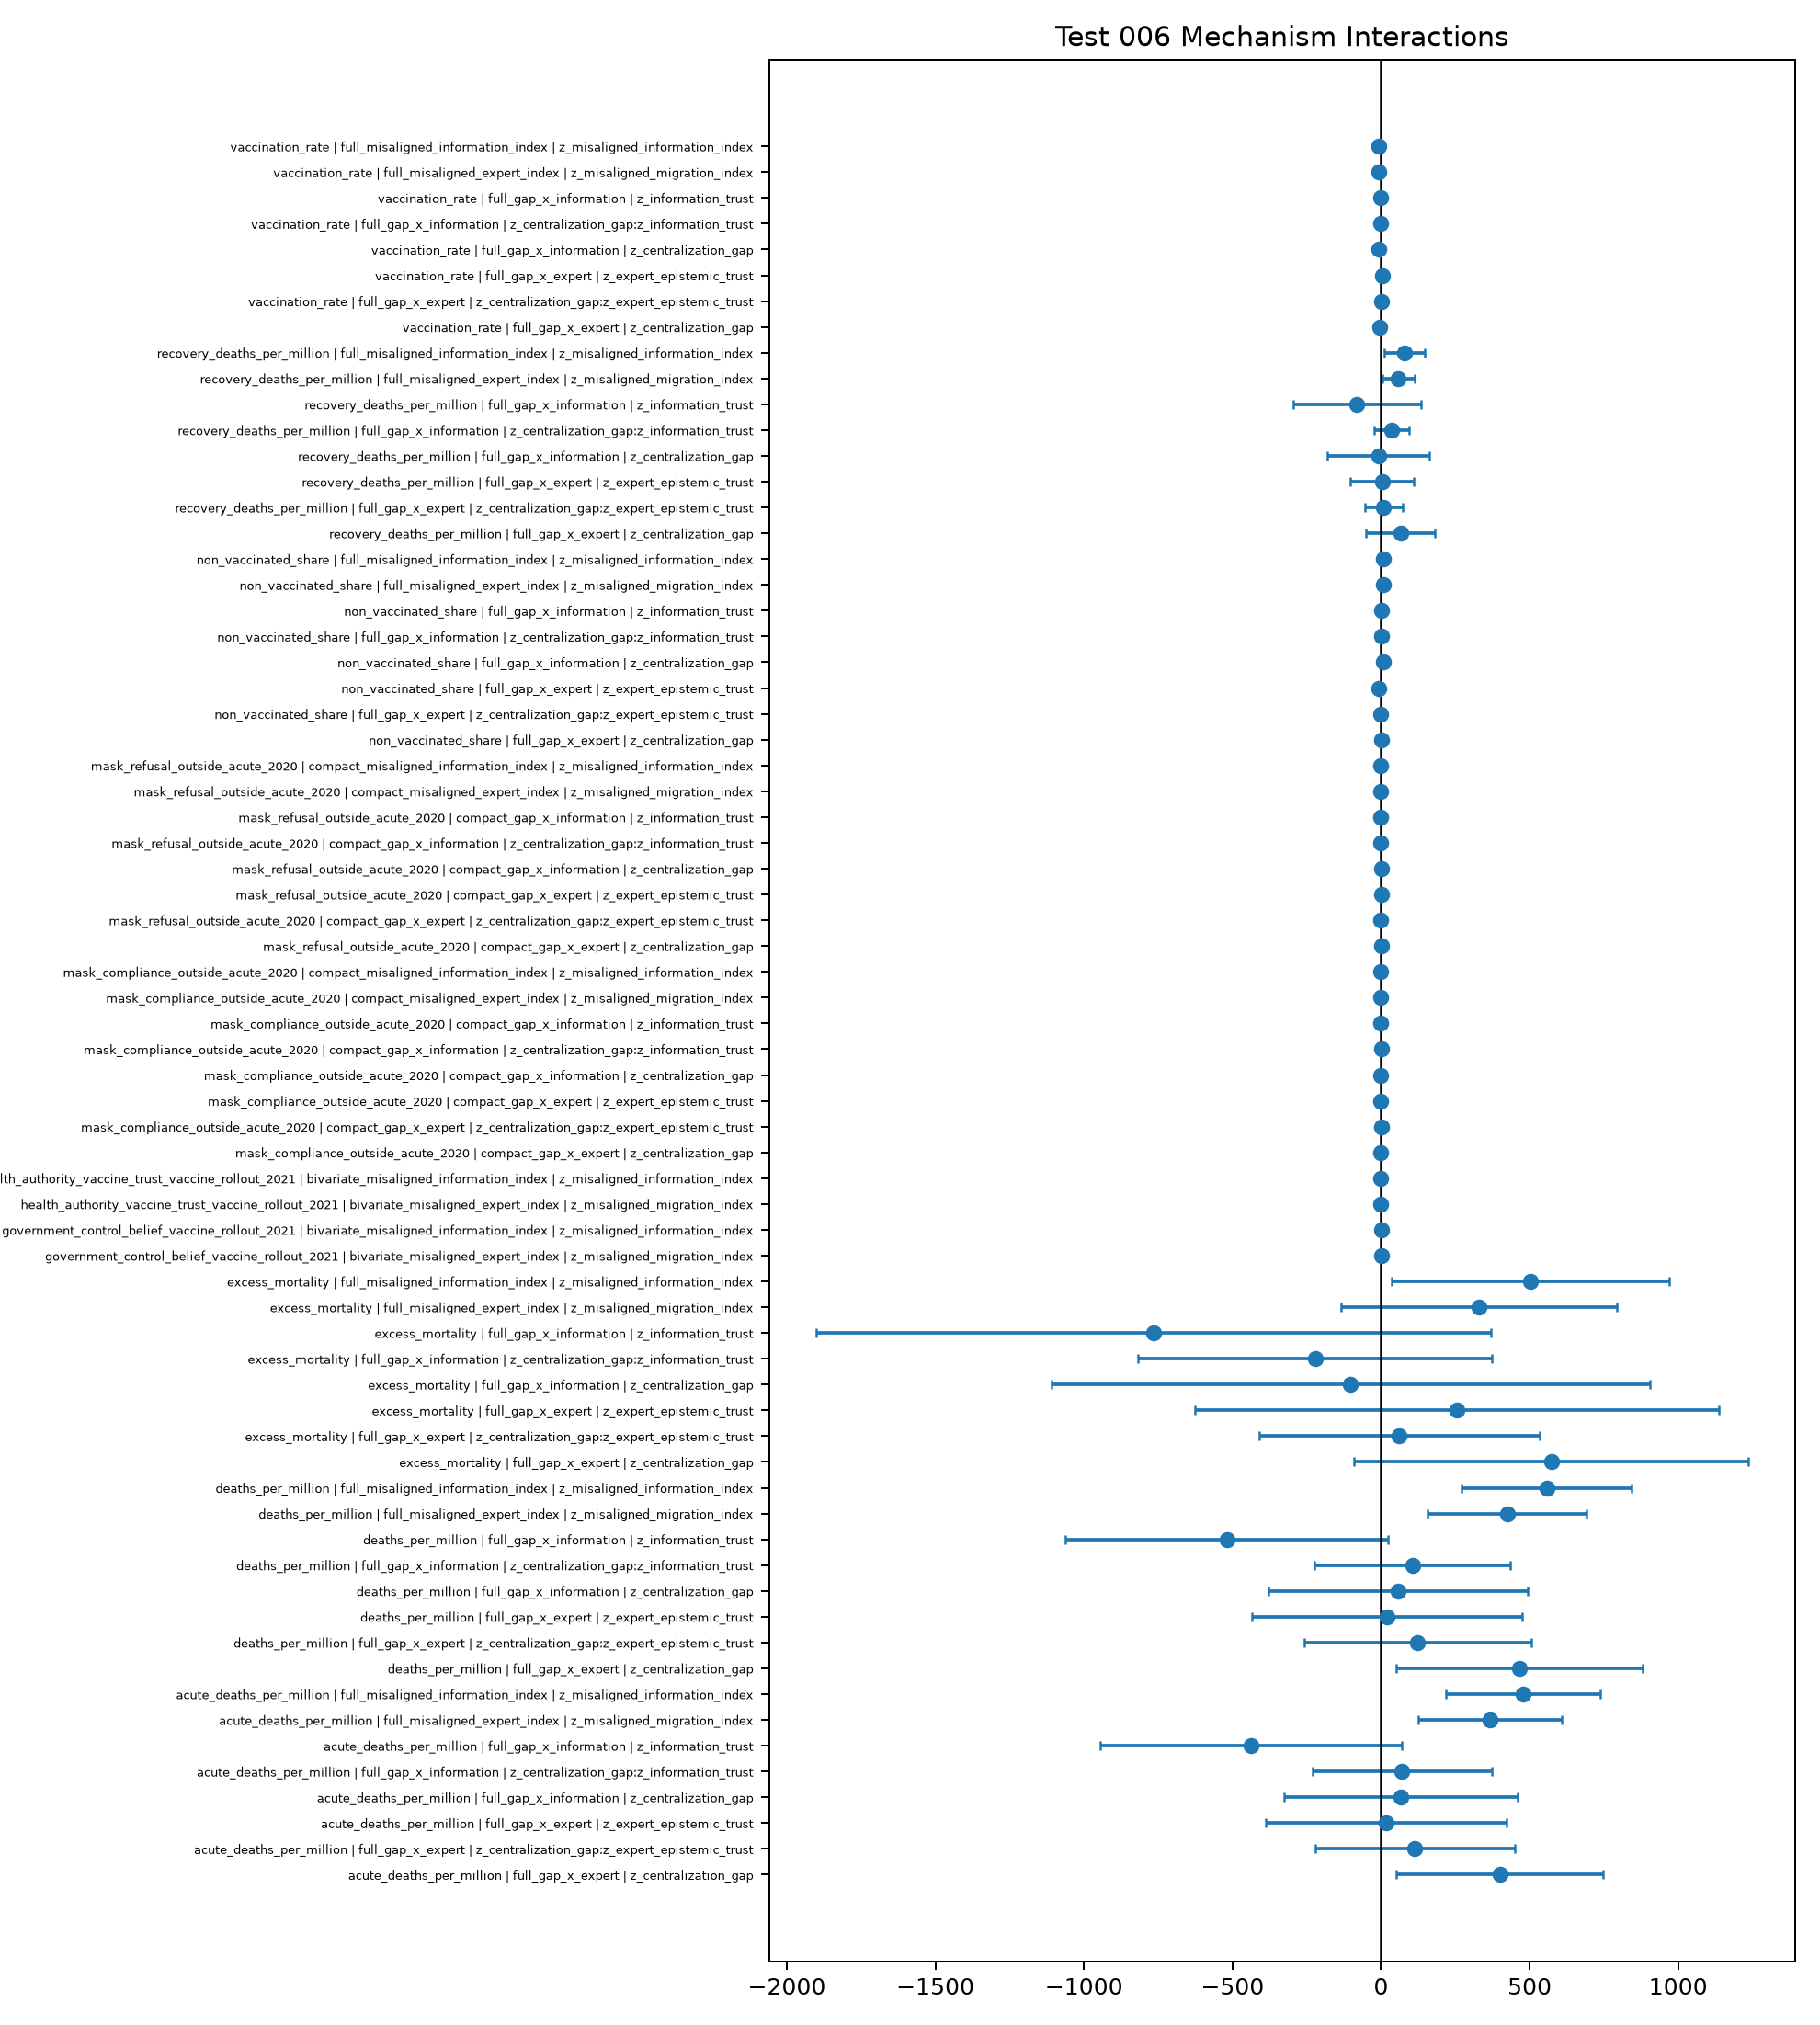
\includegraphics[width=0.92\linewidth]{../../research/aethercore-test-001/figures/test006_mechanism_coefficients.png}
  \caption{\textbf{Mechanism coefficients.} Misalignment indices produced stronger and more consistent patterns than simple interaction terms.}
\end{figure}

\section{Scientific Interpretation}

\subsection{What the Results Support}

The test series supports six cautious claims.

\begin{enumerate}
  \item \textbf{Trust variables have measurable predictive value.} Trust-density and trust-taxonomy variables improved prediction of several COVID shock outcomes after conventional controls.
  \item \textbf{The location of trust matters.} Centralized institutional trust, expert trust, information trust, and decentralized social trust are not interchangeable.
  \item \textbf{Centralized institutional trust appears protective.} Countries with higher centralized institutional trust tended to show lower deaths per million, lower acute deaths, lower recovery deaths, and lower excess mortality.
  \item \textbf{Centralization gap appears risky.} Countries where decentralized social trust exceeded centralized institutional trust tended to show higher deaths, lower vaccination uptake, higher non-vaccinated share, and higher government-control belief in exploratory behavioral models.
  \item \textbf{Alignment appears more informative than total trust.} Misalignment indices performed more consistently than simple interaction terms, suggesting that divergence among trust channels may be a measurable fragmentation signal.
  \item \textbf{Trust likely interacts with capacity.} State-capacity controls did not erase the main signal, but regional and timing sensitivity indicate that trust cannot be studied apart from institutional competence and context.
\end{enumerate}

\subsection{What the Results Do Not Prove}

The results do not prove that distrust in centralized institutions caused COVID deaths. They also do not prove that decentralized communities are harmful. Several alternative explanations remain plausible:

\begin{itemize}
  \item high death rates may reduce trust rather than the reverse;
  \item trust may proxy institutional competence;
  \item unobserved political, regional, cultural, or media-system variables may drive both trust and outcomes;
  \item survey timing may contaminate trust measures;
  \item ecological country-level relationships may not hold at the individual level.
\end{itemize}

The strongest warranted conclusion is not causal proof, but research-grade signal.

\subsection{How the Findings Refine AetherCore}

The empirical findings refine the AetherCore Framework in three ways.

First, they weaken any naive version of the theory that treats trust as a single substance. Trust is not like water poured evenly through a society. It is more like a network of channels. A person may trust family but not government, doctors but not media, local leaders but not national agencies, or science in general but not a specific policy. These distinctions matter.

Second, they shift attention from trust quantity to trust topology. The central question is not whether a society has high or low trust in the abstract. The central question is whether trust channels connect local communities to competent institutions and reliable knowledge during uncertainty.

Third, they make the theory more falsifiable. AetherCore should not predict that every form of trust improves every outcome. It should predict that coherent trust alignment improves coordination while trust misalignment increases fragmentation risk. This is a sharper and more vulnerable claim, which makes it scientifically better.

\subsection{Layman's Interpretation of the Scientific Result}

The simplest interpretation is this: during COVID, people needed to decide whom to listen to. Some countries had enough trust in public institutions, experts, and information channels that guidance could move through the society with less friction. Other countries had strong social bonds but weaker confidence in central institutions or expert channels. In those places, people may have turned more heavily toward local networks, friend groups, alternative media, or identity communities.

That shift is understandable. People often turn to those closest to them when central systems feel untrustworthy. But in a pandemic, the quality of information matters enormously. If trusted local networks spread accurate guidance, they can save lives. If they spread suspicion, delay, or misinformation, they can increase risk. The AetherCore refinement is that trust is powerful because it coordinates behavior. The danger is that coordination can move in the wrong direction.

\section{Misconceptions to Avoid}

\subsection{Misconception 1: The Goal Is Final Proof}

Final proof is not the goal. Scientific progress occurs through progressively better tests, not through one decisive result. The correct goal is to make AetherCore claims measurable, falsifiable, comparable, and refinable.

\subsection{Misconception 2: All Trust Is Good}

The results do not support a simple ``trust good, distrust bad'' interpretation. Trust can coordinate accurate action or inaccurate action. A community can trust reliable experts, or it can trust misinformation networks. Trust is a coordination amplifier; what it amplifies depends on the epistemic environment.

\subsection{Misconception 3: Decentralized Trust Is the Problem}

Decentralized social trust is not inherently harmful. Families, neighborhoods, religious communities, mutual aid networks, and local associations are essential to resilience. The risk appears when decentralized trust is disconnected from central institutions, expert systems, and information-integrity channels during a high-uncertainty crisis.

\subsection{Misconception 4: Institutional Trust Means Blind Obedience}

Institutional trust should not be interpreted as submission to authority. Healthy institutional trust means that institutions are perceived as legitimate, competent, accountable, and aligned with public welfare. Blind trust can be dangerous. Earned trust is infrastructure.

\subsection{Misconception 5: Non-Vaccinated Share Equals Anti-Vaxxer Identity}

Non-vaccinated share is an uptake outcome, not an identity measure. It may reflect access, availability, policy, logistics, eligibility, medical contraindications, hesitancy, refusal, or distrust. Behavioral survey items provide better refusal proxies, but with smaller sample size.

\subsection{Misconception 6: Correlation Means Causation}

The models are observational. They estimate associations and incremental predictive value. They do not establish causation. The next phase requires longitudinal designs, pre-pandemic trust baselines, individual-level behavior data, and stronger quasi-experimental strategies.

\section{Conclusions}

The AetherCore empirical sequence began with a broad question: does trust density predict COVID shock response after conventional controls? The answer is provisionally yes, but the stronger conclusion is more precise.

The best current formulation is:

\begin{quote}
COVID shock outcomes were associated not merely with the amount of trust in a society, but with the topology of trust. Higher centralized institutional trust was generally associated with better outcomes. Higher decentralized social trust relative to centralized institutional trust was associated with worse outcomes, especially when expert and information trust were weak.
\end{quote}

This formulation is more scientifically useful than the original broad claim. It is also more aligned with the AetherCore Framework. The issue is not trust as an isolated variable. The issue is relational coherence among trust channels. A society may possess strong community trust, but if that trust is epistemically isolated from reliable institutions, expert knowledge, and information-integrity systems, it may coordinate resistance rather than recovery.

In AetherCore language, the failure mode is not simply distrust. It is trust migration under conditions of institutional legitimacy collapse and epistemic fragmentation.

The refined AetherCore hypothesis should therefore be carried forward as a trust-alignment theory:

\begin{quote}
\textbf{Coherent trust density improves shock recovery when interpersonal trust, decentralized community trust, expert trust, information trust, institutional trust, and state capacity remain aligned. Misaligned trust may amplify fragmentation even when some forms of social trust are strong.}
\end{quote}

This is a better hypothesis because it explains both sides of the evidence. It explains why institutional and expert trust were often protective. It also explains why decentralized trust was not automatically protective. The issue is not that communities are dangerous. The issue is that communities can become isolated from reliable knowledge when institutions lose legitimacy. A coherent civilization does not force people to choose between community and institution. It builds trustworthy bridges between them.

\section{Further Research Areas}

\subsection{Pre-Pandemic Trust Baselines}

Future tests should replicate the analysis using trust measures collected strictly before COVID-19. Earlier WVS waves, European Social Survey, Latinobarometro, Afrobarometer, Asian Barometer, Gallup World Poll, and country-specific longitudinal surveys may provide stronger temporal ordering.

\subsection{Individual-Level Multilevel Modeling}

Country-level models risk ecological fallacy. The next major step is individual-level modeling:

\[
\text{Behavior}_{ij} =
f(\text{individual trust}_{ij},
\text{country trust topology}_{j},
\text{controls}_{ij},
\text{controls}_{j}).
\]

This would test whether individuals with low institutional trust and high local-network reliance were more likely to refuse vaccination, avoid masks, or endorse government-control beliefs.

\subsection{Information Ecology}

The information-trust proxy used here is weak. Future work should add:

\begin{itemize}
  \item press freedom indices;
  \item media polarization measures;
  \item misinformation exposure data;
  \item social media penetration;
  \item platform trust;
  \item V-Dem digital society indicators;
  \item fact-checking infrastructure.
\end{itemize}

\subsection{State Capacity and Legitimacy}

Institutional trust may reflect real competence. Future work should separate:

\begin{itemize}
  \item trust as public psychology;
  \item state capacity as institutional performance;
  \item legitimacy as perceived moral authority;
  \item accountability as constraint on institutional abuse.
\end{itemize}

This distinction matters because the policy implication is not ``increase trust messaging.'' It is to build institutions that deserve trust.

\subsection{Shock Generalization}

COVID is only one shock. The trust-migration hypothesis should be tested against:

\begin{itemize}
  \item natural disasters;
  \item financial crises;
  \item public-health campaigns;
  \item election legitimacy crises;
  \item climate adaptation events;
  \item infrastructure failures;
  \item cyberattacks and information shocks.
\end{itemize}

\subsection{Trust Recovery Dynamics}

Future research should examine not only shock performance, but trust repair:

\begin{itemize}
  \item How quickly does institutional trust recover after failure?
  \item Which institutions recover trust fastest?
  \item Does transparent admission of error improve recovery?
  \item Do decentralized communities reconnect to institutions after crisis, or remain separated?
\end{itemize}

\subsection{Trust Alignment Metrics}

The next research cycle should develop and compare multiple trust-alignment metrics. Candidate measures include:

\begin{itemize}
  \item standard deviation across trust channels;
  \item centralization gap;
  \item expert misalignment index;
  \item information misalignment index;
  \item institutional legitimacy gap;
  \item weighted alignment scores tailored to specific shock types;
  \item latent-factor models distinguishing trust level from trust coherence.
\end{itemize}

The key test is whether alignment metrics outperform simple trust-level metrics. If alignment consistently predicts shock recovery better than total trust, the AetherCore claim becomes more specific and empirically stronger.

\subsection{Positive and Negative Trust}

Future work should distinguish between \textit{positive trust} and \textit{negative trust}. Positive trust connects participants to accurate information, competent institutions, accountable leadership, and constructive cooperation. Negative trust connects participants to closed information loops, identity-protective misinformation, or resistance networks that intensify risk.

This distinction is philosophical and empirical. Philosophically, it means trust is not automatically virtuous. Scientifically, it means trust must be evaluated by what it connects to, what behavior it coordinates, and whether the coordinated behavior improves or worsens outcomes.

\section{Recommended Strategy Before Publication}

\subsection{Freeze the Refined Main Hypothesis}

Before publication, the paper should explicitly state that the broad trust-density hypothesis has been refined. The next confirmatory version should not claim:

\begin{quote}
More trust always predicts better outcomes.
\end{quote}

It should claim:

\begin{quote}
Better aligned trust architectures predict better shock recovery, while misalignment between decentralized social trust, institutional trust, expert trust, and information trust predicts fragmentation risk.
\end{quote}

This distinction prevents the theory from becoming too loose. If all positive trust results and all negative trust results are interpreted as support, the theory becomes unfalsifiable. The refined version has clearer risk: if trust-alignment measures do not improve prediction after controls, or if they perform worse than ordinary material-capacity models, the AetherCore trust-alignment claim should be weakened.

\subsection{Freeze a Main Model}

The paper should define one primary confirmatory model before additional exploration:

\begin{align*}
\text{Deaths per Million} \sim{}&
\text{Controls} +
\text{Centralized Institutional Trust} \\
&+
\text{Decentralized Social Trust} +
\text{Expert Trust} +
\text{Information Trust}.
\end{align*}

A second pre-specified model should test:

\[
\text{Deaths per Million} \sim
\text{Controls} +
\text{Centralization Gap}.
\]

Exploratory models can then examine misalignment indices and behavioral outcomes.

\subsection{Add a Lay Summary}

The repo PDF should include a one-page lay summary. The summary should say:

\begin{quote}
The study does not show that people should blindly trust central authorities. It shows that crisis response appears stronger when communities, institutions, experts, and information systems remain connected. When people trust their local networks but distrust institutions and experts, coordination can move away from public-health guidance. That pattern may increase fragmentation during a shock.
\end{quote}

This language is important because the results can be misread politically. The science is not an argument for centralization as domination. It is an argument for trustworthy institutions and connected communities.

\subsection{Prepare a Replication Package}

The repository should include:

\begin{itemize}
  \item raw-data download scripts;
  \item manual WVS instructions and licensing note;
  \item processed datasets;
  \item analysis scripts for Tests 001--006;
  \item model output CSVs;
  \item figures;
  \item a reproducibility README;
  \item session/package versions;
  \item a data dictionary.
\end{itemize}

\subsection{Add a Data Dictionary}

The repo PDF should include a concise data dictionary mapping every major variable to:

\begin{itemize}
  \item source dataset;
  \item original variable name;
  \item transformation;
  \item interpretation;
  \item limitation.
\end{itemize}

\subsection{Add a Falsification Section}

A publishable paper should explicitly define what would weaken the claim:

\begin{itemize}
  \item centralization gap loses direction under pre-pandemic trust data;
  \item trust-alignment indices fail to outperform simple trust-level variables;
  \item effects vanish under stronger state-capacity controls;
  \item individual-level models do not reproduce the country-level pattern;
  \item misinformation/information variables explain the entire effect;
  \item other shocks do not show similar trust-topology dynamics.
\end{itemize}

\subsection{Add a Pre-Registration Appendix}

The next version should include a pre-registration appendix specifying:

\begin{itemize}
  \item primary outcomes;
  \item primary trust predictors;
  \item control variables;
  \item exclusion rules;
  \item robustness checks;
  \item correction strategy for multiple comparisons.
\end{itemize}

\section{What Else Should Be Included in the Repo PDF?}

The empirical repo PDF should include the following artifacts beyond the narrative white paper:

\begin{enumerate}
  \item \textbf{Executive summary}: one page with main findings, limitations, and next steps.
  \item \textbf{Theory-to-variable map}: how AetherCore concepts map to measurable variables.
  \item \textbf{Dataset provenance table}: source URLs, download dates, file names, and licenses.
  \item \textbf{Variable dictionary}: original variables, transformations, constructed variables, and caveats.
  \item \textbf{Model specification appendix}: exact formulas for every test.
  \item \textbf{Full regression tables}: not only selected coefficients.
  \item \textbf{Robustness appendix}: log, winsorized, rank, robust regression, and leave-one-out outputs.
  \item \textbf{Figures appendix}: scatterplots, coefficient plots, heatmaps, and influence plots.
  \item \textbf{Limitations and falsification appendix}: explicit conditions that would weaken or reject the trust-migration claim.
  \item \textbf{Future research roadmap}: data acquisition targets, replication strategy, and pre-registration plan.
  \item \textbf{Reproducibility instructions}: how to recreate all outputs from raw data.
  \item \textbf{Ethics note}: avoid stigmatizing communities; distinguish distrust caused by real institutional failure from misinformation-driven distrust.
\end{enumerate}

\section*{Final Statement}
\addcontentsline{toc}{section}{Final Statement}

The first empirical AetherCore test sequence found a meaningful signal: trust topology appears associated with crisis response. The most scientifically defensible claim is not that trust universally improves outcomes, nor that centralized institutions should be trusted uncritically, nor that decentralized communities are dangerous. The defensible claim is subtler and stronger:

\begin{quote}
In a systemic shock, societies appear more resilient when centralized institutions, expert systems, information channels, and decentralized communities remain coherently aligned. When trust migrates away from central institutions into decentralized networks while expert and information trust are weak, coordination may fragment and mortality risk may rise.
\end{quote}

This is the next AetherCore research frontier: not trust as sentiment, but trust as system architecture.

\end{document}
